Wie bereits in Kapitel \ref{sec:global_curveball} erwähnt, muss die disjunkte Nachbarschaft
der beiden Knoten $u$ und $v$ bekannt sein, um einen \ct{} auf diesen Knoten $u$ und $v$
auszuführen. Der \ct{} besteht dann darin, diese Knoten aus $N_{d}(u,v)$ zu durchmischen.
Deshalb beschäftigen wir uns zuerst damit, wie man die disjunkte Nachbarschaft bestimmt.

%%%%%%%%%%%%%%%%%%%%%%%%%%%%%%%%%%%%%%%%%%%%%%%%%%%%%%%%%%%%%%%%%%%%%%%%
%%%%%% COMMON NEIGHBORS
%%%%%%%%%%%%%%%%%%%%%%%%%%%%%%%%%%%%%%%%%%%%%%%%%%%%%%%%%%%%%%%%%%%%%%%%

\section{Bestimmung der disjunkten Nachbarschaft}
\label{sec:common}
Gesucht sind alle Knoten aus der disjunkten Nachbarschaft der Knoten $u$ und $v$.
Nach Definition \ref{def:common_disjoint} liegt jeder Knoten aus den Nachbarschaften $N(u)$ und $N(v)$ 
entweder in der disjunkten oder in der gemeinsamen Nachbarschaft. Das Ziel besteht also darin, 
für jeden Knoten aus $N(u) \cup N(v)$ zu entscheiden, ob er zu $N_{d}(u,v)$ oder $N_{c}(u,v)$ gehört.
\\

Die Nachbarschaften $N(u)$ und $N(v)$ liegen jeweils
in einem Array vor (siehe Abschnitt \ref{sec:datenstruktur}). Der Übersichtlichkeit 
wegen werden wir die beiden
Arrays ebenfalls mit $N(u)$ und $N(v)$ bezeichnen. Aufgabe ist es,
 für jedes Element aus den beiden Arrays zu entscheiden,
ob es entweder in beiden Arrays vorkommt oder nur in einem von den beiden. Dafür 
gibt es verschiedene algorithmische Ansätze.
\\

Als ersten naiven Ansatz könnte man für jedes Element $x \in N(u)$ mittels
 linearer Suche überprüfen, ob $x$ auch in $N(v)$ enthalten ist. Hierfür ergibt sich eine Laufzeit von
$\O(|N(u)|\cdot|N(v)|)$. Dies ist aber problematisch, da wir 
im Falle von massiven Graphen davon ausgehen können, dass die Nachbarschaften
 groß werden. 
\\

Ein Lösungsansatz besteht darin, beide Arrays aufsteigend zu sortieren. 
Um herauszufinden,
welche Werte in beiden Arrays vorkommen, muss man ---analog zu Merge--- lediglich $N(u)$ und $N(v)$
gleichzeitig linear durchlaufen. Somit muss man jedes 
Element der beiden Arrays ---nach dem Sortieren--- 
nur einmal betrachten, was offensichtlich zu einer verbesserten Laufzeit im Vergleich zum naiven
Ansatz führt. Man erhält damit eine Laufzeit von $\O(|N(u)|\cdot \log (|N(u)|)  + |N(v)|\cdot\log(|N(v)|))$. 
Diese Variante wird im Folgenden als \SorSor{} bezeichnet. 
\\

Die Laufzeit von \SorSor{} wird dabei vom Sortieren dominiert. Daher führen wir eine Variante ein, 
die wir \fett{vorsortiert} nennen. Bei dieser Variante nehmen wir an, dass
die Arrays immer im sortierten Zustand vorliegen. Somit würde bei \SorSor{} das Sortieren wegfallen
und man müsste die beiden Arrays nur noch linear durchlaufen. 
Dies verbessert die Laufzeit auf $\O(|N(u)| + |N(v)|)$. 
Es ist jedoch nicht offensichtlich, dass die Variante zu einer insgesamt besseren Laufzeit eines
\ct{es} führt, da ein \ct{} schließlich auch noch aus dem Durchmischen der disjunkten Nachbarschaft besteht.
Dadurch könnte die angenommene Sortierung verletzt werden, weshalb man am Ende des \ct{es} nochmal sortieren
müsste.
\\

Wie wir in Kapitel \ref{sec:entscheidung} sehen werden, 
ist \SorSor{} mit der Vorsortierung Teil der Variante, welche das beste Laufzeitverhalten aufweist.
Deswegen gehen wir an dieser Stelle 
noch einmal genauer auf diese Methode ein, indem wir sie in Pseudocode
beschreiben.
\begin{algorithm}
  \caption{SortSort}\label{algo:sortsort}
  \begin{algorithmic}[1]
    \Procedure{SortSort}{$u,v$}
	  \State U $ \gets N(u)$ \Comment{vorsortierte Nachbarschaft von u}
	  \State V $ \gets N(v)$ \Comment{vorsortierte Nachbarschaft von v}
	  \State common $\gets $  [ ] \Comment{anfänglich leeres Array der gemeinsamen Nachbarschaft}
	  \State disjoint $\gets $ [ ]\Comment{anfänglich leeres Array der disjunkten Nachbarschaft}

	  \State nu $\gets 0$ \Comment{Zähler für U}
	  \State nv $\gets 0$ \Comment{Zähler für V}
      
      \While{(nu < |U|) and (nv < |V|)}
        \If{U[nu] < V[nv]}
			\State disjoint.\texttt{append(}U[nu]\texttt{)} \Comment{Füge das Element in disjoint ein}
			\State nu ++
			\ElsIf{U[nu] > V[nv]}
				\State disjoint.\texttt{append(}V[nv]\texttt{)} \Comment{Füge das Element in disjoint ein}
				\State nv ++
			\ElsIf{U[nu] == V[nv]}
				\State common.\texttt{append(}U[nu]\texttt{)} \Comment{Füge das Element in common ein}
				\State nu ++
				\State nv ++
        \EndIf
      \EndWhile
      \If{nu $\neq$ |U|} \Comment{Die restlichen Elemente sind disjunkte Nachbarn}
			\State disjoint.\texttt{append(}U[nu], U[nu+1], \dots\texttt{)}
			\Else{}
			\State disjoint.\texttt{append(}V[nv], V[nv+1], \dots\texttt{)}
      \EndIf
      \State \textbf{return} common, disjoint
   \EndProcedure
  \end{algorithmic}
  \label{algo:sortsort}
\end{algorithm}
\\

Die Variante \SorSor{} lässt sich leicht abwandeln, indem wir nur eines der beiden Arrays sortieren.
Auf diese Weise können wir die Laufzeit des einen Sortiervorgangs sparen. Sortieren
wir das größere Array (ohne Beschränkung der Allgemeinheit $N(v)$), bezeichnen wir die Variante als \SorSea{}. Um zu erkennen, 
welche Elemente zur gemeinsamen und welche zur disjunkten Nachbarschaft gehören, kann man für jeden
Knoten aus $N(u)$ per binärer Suche in logarithmischer Zeit prüfen, ob der Knoten auch in $N(v)$ vorhanden ist.
Damit ergibt sich eine Laufzeit von $\O(|N(v)| \cdot \log(|N(v)|) + |N(u)| \cdot \log(|N(v)|)$. Analog dazu
nennen wir die Variante, in der das kleinere Array sortiert wird, \SeaSor. 
Auch hier könnte die Variante mit Vorsortierung einen Vorteil bringen, da die Laufzeit
für das Sortieren entfällt.
\\

Eine weitere Methode, um viele Werte schnell zu durchsuchen, bietet die Datenstruktur \texttt{set}, welche
einem binären Suchbaum entspricht, beispielsweise einem Rot-Schwarz-Baum.
Dabei wird jedes Element des einen Arrays in den Suchbaum eingefügt. 
Für jedes Element des anderen Arrays kann nun in logarithmischer
Zeit bestimmt werden, ob es im \texttt{set} und somit auch im ursprünglichen Array vorhanden ist.
Somit erhält man die identischen asymptotischen Laufzeiten wie bei der Verwendung der
binären Suche. Je nach Implementierung des Suchbaums könnte es aber auch zu einer verbesserten
Laufzeit führen. 
Für diese Möglichkeit gibt es ebenfalls zwei 
analoge Varianten, nämlich \SetSea, bei der die Elemente des größeren Arrays in das \texttt{set} eingefügt werden
und \SeaSet, bei der das kleinere Array zum \texttt{set} hinzugefügt wird.
Im Gegensatz zur Methode mit der binären Suche führt das Verwenden der vorsortierten Variante in diesem Fall
nicht zu einer asymptotisch besseren Laufzeit. Dies liegt daran, da es asymptotisch
gesehen für das Erstellen eines Binärbaums keinen Unterschied macht, ob die Werte sortiert sind oder nicht.
Je nach Implementierung des Suchbaums könnte es trotzdem zu einem Laufzeitvorteil führen, 
wenn die Nachbarschaften bereits sortiert sind.
\\

Die letzte Methode, die wir an dieser Stelle betrachten werden,
ist die Verwendung der Datenstruktur \texttt{unordered\_set}. Diese ist \texttt{set} sehr ähnlich, jedoch mit
dem Unterschied, dass die Werte nicht in geordneter Reihenfolge gespeichert werden, sondern
in einer Hash-Tabelle. Ein Vorteil einer Hash-Tabelle liegt darin, 
dass das Einfügen und Suchen von Elementen
erwartet in konstanter Zeit erfolgt.
Ebenfalls gibt es hierbei wieder die Varianten, 
in denen entweder das größere Array in das \texttt{unordered\_set} eingefügt wird (\USetSea) 
oder das kleinere (\SeaUSet).{}
Asymptotisch ergibt sich in beiden Fällen eine erwartete Laufzeit von $\O(|(N(u)| + |N(v)|)$.
Diese Laufzeit hängt jedoch stark von der Implementierung und dem Füllgrad  der Hash-Tabelle ab. 
Schließlich werden wir auch bei den letzten beiden Methoden prüfen,
 ob die Vorsortierung eventuell zu einer besseren Laufzeit führt.
\\

Zusammenfassend betrachten wir also insgesamt sieben verschiedene Möglichkeiten, um die disjunkte
und gemeinsame Nachbarschaft zu berechnen. Für jede dieser Varianten prüfen wir zusätzlich,
ob die vorsortierte Variante zu einer verbesserten Laufzeit führt oder ob es sich
nicht lohnt, diese aufrechtzuerhalten.


%%%%%%%%%%%%%%%%%%%%%%%%%%%%%%%%%%%%%%%%%%%%%%%%%%%%%%%%%%%%%%%%%%%%%%%%
%%%%%% Nachbarn Tauschen
%%%%%%%%%%%%%%%%%%%%%%%%%%%%%%%%%%%%%%%%%%%%%%%%%%%%%%%%%%%%%%%%%%%%%%%%

\section{Tauschen der Nachbarn}
\label{sec:trade}
Im vorherigen Teil wurde beschrieben, wie man die gemeinsame und die disjunkte Nachbarschaft zweier Knoten
$u$ und $v$ bestimmt. Nun beschäftigen wir uns damit, wie man die Knoten der disjunkten Nachbarschaft zufällig tauscht. Als Eingabe 
stehen die Arrays $N_{d}(u,v)$, welches alle Knoten aus der disjunkten Nachbarschaft enthält
und $N_{c}(u,v)$, das die gemeinsamen Nachbarn enthält, zur Verfügung. Weiterhin seien $\text{deg}(u)$ und
$\text{deg}(v)$ die ursprünglichen Knotengrade. Zusätzlich definieren wir uns die Mengen
$D_{u} = N_{d}(u,v) \cap N(u)$, in der die disjunkten Nachbarn von Knoten $u$ liegen, 
und $D_{v} = N_{d}(u,v) \cap N(v)$, in der die disjunkten Nachbarn von $v$ liegen. Die anfänglich
leeren Arrays, in denen die Ausgabe ---also die neuen Nachbarschaften von $u$ und $v$--- zurückgegeben 
werden soll, bezeichnen wir als $N'(u)$ und $N'(v)$.
Wir betrachten zwei unterschiedliche Möglichkeiten.
\\

Die erste Idee besteht darin,  
das Array der disjunkten Nachbarschaft zufällig zu permutieren, sodass jedes Element an 
einer zufälligen Position steht. Um nun die beiden \glqq neuen\grqq{} Nachbarschaften von $u$ und $v$ zu erstellen,
werden zuerst die Knoten aus der gemeinsamen Nachbarschaft in die leeren Arrays $N'(u)$ und $N'(v)$ kopiert.
Dann werden die ersten $|D_{u}|$ Elemente aus dem permutierten Array in $N'(u)$ kopiert, die restlichen
in $N'(v)$. Somit haben die Nachbarschaften durch den Tausch ihre 
ursprüngliche Größe nicht verändert und es gilt $|N'(u)| = \deg(u)$ und
$|N'(v)| = \deg(v)$.
Zur besseren Veranschaulichung ist in Abbildung \ref{fig:trade_shuffle} ein Beispiel dargestellt.
%
%
%%%%% Trade mit Permuatation
\begin{figure}
\centering
  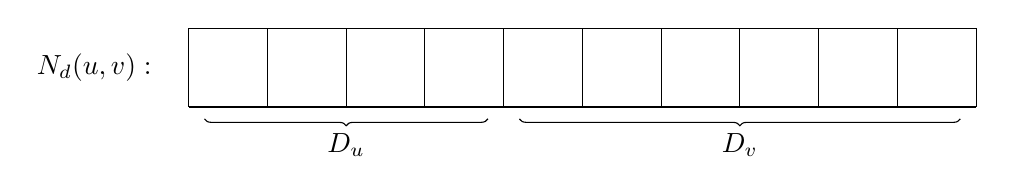
\begin{tikzpicture}[decoration=brace]
    % Die Grundlinie:
    \draw(0,0)--(10,0);
    \draw(0,1)--(10,1);

    % Striche und Beschriftung in Abständen 0, 2, 4, 6, ...
    \foreach \x/\xtext in {0,1,2,3,4,5,6,7,8,9,10}
      \draw(\x,0)--(\x,1) node[below] {};
      
    % untere geschweifte Klammer mit Text darunter:
    \draw[decorate, yshift=-1ex] (3.8,0) -- node[below=0.4ex] {$D_{u}$} (0.2,0);

    \draw[decorate, yshift=-1ex] (9.8,0) -- node[below=0.4ex] {$D_{v}$} (4.2,0);

\node[] at (-1.2, 0.5)     (5)     {$N_{d}(u,v):$};

  \end{tikzpicture}
  \caption[Beispiel eines Tausches der disjunkten Nachbarschaft mit der Variante Permutation]{Beispiel für einen Tausch mit der Variante \perm. Dabei wird das Array der 
  disjunkten Nachbarschaft $N_{d}(u,v)$ zufällig permutiert. Die ersten $|D_{u}|$ Elemente werden der Nachbarschaft
  von $u$ zugeordnet, die restlichen $|D_{v}|$ zur Nachbarschaft von $v$. }
  \label{fig:trade_shuffle}
\end{figure}
%
%
%
\\

Bei diesem Verfahren fällt  jedoch auf, dass einige Elemente beim Permutieren unnötig vertauscht werden.
Für jedes Element ist es eigentlich nur entscheidend, ob es unter den ersten $|D_{u}|$  liegt (also zum Array
$N'(u)$ hinzugefügt wird) oder nicht. Auf welcher Position es genau in 
diesen Bereichen liegt, ist nicht relevant. Ohne Beschränkung der Allgemeinheit gelte 
$N(u) \le N(v)$. Dann kann man
also die Laufzeit dieser Variante verbessern, indem nicht das ganze Array der disjunkten Nachbarschaft zufällig permutiert 
wird, sondern nur die ersten $|D_{u}|$ Elemente zufällig gewählt werden.
 Dies setzt die Funktion 
\texttt{random\_bipartition\_shuffle} um.
\\

Ein Nachteil dieser Methode besteht jedoch darin, dass durch das zufällige Vertauschen die beiden resultierenden Arrays
$N'(u)$ und $N'(v)$ im Allgemeinen nicht mehr sortiert sind. 
Damit wird die im Abschnitt \ref{sec:common} beschriebene
Variante eventuell verletzt. Möchte man die Vorsortierung aufrechterhalten, müssen somit die beiden Arrays
in einem letzten Schritt nochmals sortiert werden.
Wir nennen diese Variante \perm.
\\

Die zweite Möglichkeit, die wir betrachten, werden wir als \distr{} bezeichnen.
Die Idee besteht dabei, dass wir über jedes Element des Arrays $N_{d}(u,v)$ iterieren und 
die Wahrscheinlichkeit $p$ berechnen, mit
der das Element in die Nachbarschaft von $u$ (beziehungsweise $v$) eingefügt werden soll. Dann wird in einem 
Bernoulli-Experiment mit Wahrscheinlichkeit $p$ ein Zufallsbit gezogen. Je nachdem welchen
Wert das Zufallsbit hat, wird das Element dann entweder in $N'(u)$ oder in $N'(v)$ kopiert. Dies wird so lange
wiederholt bis eines der beiden Arrays seine maximale Kapazität erreicht hat. 
\\

Um die Wahrscheinlichkeit zu berechnen, werden am Anfang zwei Variablen $n_u$ und $n_v$ initialisiert, 
welche den Kapazitäten der beiden Arrays $u$ und $v$ entsprechen, wenn die Elemente aus der 
gemeinsamen Nachbarschaft nicht berücksichtigt werden. Es gilt also $n_u = |D_{u}|$ und
$n_v= |D_{v}|$.
Damit hat das erste Element des Arrays $N_{d}(u,v)$ eine Wahrscheinlichkeit von $p_u = \frac{n_u}{n_u+n_v}$, dem
Array $N'(u)$ hinzugefügt zu werden und analog eine Wahrscheinlichkeit $p_v = \frac{n_v}{n_u+n_v}$, um
in $N'(v)$ zu gelangen. Offensichtlich gilt $p_u + p_v = 1$. Dann wird mit einer der beiden
Wahrscheinlichkeiten das Bernoulli-Experiment durchgeführt, wobei es irrelevant ist, welche Wahrscheinlichkeit
man dazu wählt, da $p_u$ genau die Gegenwahrscheinlichkeit von $p_v$ ist und umgekehrt. 
Wählt man beispielsweise $p_u$ und das Experiment liefert eine eins, dann wird das aktuelle Element
in $N'(u)$ kopiert. Dabei
hat sich aber offensichtlich die verbleibende Kapazität des Arrays $N'(u)$ verringert. Also muss
der Wert $n_u$ dekrementiert werden. Dies gilt analog, falls das Element in die Nachbarschaft von $v$ kopiert wird.
Somit ändern sich nach jeder Iteration die Wahrscheinlichkeiten $p_u$ beziehungsweise $p_v$.
Gilt nach irgendeinem Zeitpunkt entweder $n_u = 0$ oder $n_v = 0$, steht offenbar in einem der Arrays 
keine freie Kapazität mehr zur Verfügung. Somit werden die übrigen Elemente, die noch in $N_{d}(u,v)$ vorhanden sind, 
einfach dem anderen Array hinzugefügt.
\\

An dieser Stelle  kann man jedoch noch eine Optimierung vornehmen.
Da bei dem Bernoulli-Experiment die Wahrscheinlichkeit $p_{u}$ ---beziehungsweise $p_{v}$--- eine
rationale Zahl ist, werden zur Berechnung laufzeitintensive Gleitkommaoperationen 
benötigt. Um dies zu umgehen, kann man eine zufällige natürliche Zahl aus dem Intervall
$[0, n_{u} + n_{v})$ ziehen. Anschließend prüft man, ob die gezogene Zahl 
echt kleiner als $n_{u}$ ---beziehungsweise $n_{v}$---
ist. Wenn dies der Fall ist, fährt man genauso fort, wie wenn das Bernoulli-Experiment eine eins
zurückgibt. Auf diese Weise 
ergeben sich für ein Element die gleichen Wahrscheinlichkeiten in das jeweilige Array zu geraten, wie
beim Bernoulli-Experiment. Dabei wird aber ausschließlich Arithmetik auf ganzen Zahlen verwendet, welche
von der Recheneinheit schneller verarbeitet werden kann.
\\

Ein Vorteil dieser Methode ist, dass die in \ref{sec:common} beschriebene Variante der Vorsortierung aufrecht erhalten werden kann.
War das Array der disjunkten Nachbarschaft vor Beginn dieser Methode aufsteigend sortiert,
dann sind auch die bisherigen Elemente der Arrays $N'(u)$ und $N'(v)$ aufsteigend sortiert, da für jedes
Element nacheinander entschieden wurde, ob es zur Nachbarschaft von $u$ oder von $v$ hinzugefügt wird und dabei die
Reihenfolge der Elemente untereinander nicht verändert wurde.
\\

Zum Schluss müssen noch die gemeinsamen Nachbarn zu den Arrays $N'(u)$ und $N'(v)$ hinzugefügt werden.
Möchte man die vorsortierte Variante aufrecht erhalten, dann sind die beiden Arrays wie beschrieben schon
aufsteigend sortiert. Da auch die Elemente aus $N_{c}(u,v)$ aufsteigend sortiert sind, erhält man
die endgültigen Arrays von $N'(u)$ und $N'(v)$ durch ein Mergen mit 
$N_{c}(u,v)$. Soll die Vorsortierung jedoch
nicht aufrecht erhalten werden, reicht es aus, die Elemente aus 
$N_{c}(u,v)$ jeweils an das Ende der beiden Arrays
zu kopieren.
\\

Wird die Variante vorsortiert nicht verwendet, ergibt sich für \perm{} und \distr{}
die gleiche asymptotische Laufzeit von $\O(|N(u)| + |N(v)|)$. 
Beim Verwenden der vorsortiert Variante ändert sich die asymptotische Laufzeit für \distr{}
nicht, da das Mergen ebenfalls in linearer Zeit ausgeführt werden kann. Bei \perm{}
hingegen müssen die beiden Arrays nochmals sortiert werden. Somit entsteht
eine Laufzeit von $\O(|N(u)| \cdot \log(|N(u)|) + |N(v)| \cdot \log(|N(v)|))$.{}
\\

In Kapitel \ref{sec:entscheidung} wird sich herausstellen, dass der Algorithmus \distr{} ein Teil der
Variante ist, welche insgesamt die beste Laufzeit für einen \ct{} besitzt. Dabei wird die Variante
mit der Vorsortierung genutzt. Aus diesem Grund ist die Methode \distr{} in Form von Pseudocode
im Algorithmus \ref{algo:distr} gegeben.


\begin{algorithm}
\begin{algorithmic}[1]
\Procedure{Distribution}{common, disjoint}
	\State nu $\gets$ |U| - |common| \Comment{Kapazität von $u$}
	\State nv $\gets$ |V| - |common| \Comment{Kapazität von $v$}
	\State i = 0
	\While{i < |disjoint|}
		\State X $\sim \mathcal{B}(\frac{\text{nu}}{\text{nu}+\text{nv}})$  \Comment{Zufallsbit Bernoulli verteilt mit Wahrscheinlichkeit $\frac{nu}{nu+nv}$}

		\If{X==1}
			\State U.\texttt{append(}disjoint[i]\texttt{)} \Comment{Füge das Element in U ein}
			\State i++
			\State nu- - \Comment{aktualisiere die Kapazität}
		\Else{} 
			\State V.\texttt{append(}disjoint[i]\texttt{)}\Comment{Füge das Element in V ein}
			\State i++
			\State nv- -\Comment{aktualisiere die Kapazität}
		\EndIf{}
	\EndWhile{}	
	\State U.\texttt{merge(}common\texttt{)} \Comment{Merge U mit der gemeinsamen Nachbarschaft}
	\State V.\texttt{merge(}common\texttt{)} \Comment{Merge V mit der gemeinsamen Nachbarschaft}
	\State \textbf{return} U, V
\EndProcedure
\end{algorithmic}
	\caption{Distribution}
	\label{algo:distr}
\end{algorithm}





%%%%%%%%%%%%%%%%%%%%%%%%%%%%%%%%%%%%%%%%%%%%%%%%%%%%%%%%%%%%%%%%%%%%%%%%
%%%%%% Global Curveball Tausch
%%%%%%%%%%%%%%%%%%%%%%%%%%%%%%%%%%%%%%%%%%%%%%%%%%%%%%%%%%%%%%%%%%%%%%%%


\section{\ct}
Wie schon in Abschnitt \ref{sec:global_curveball} beschrieben, 
besteht ein \ct{} auf zwei verschiedenen Knoten $u, v \in V$  ($u\neq v$) daraus, die 
gemeinsame und disjunkte Nachbarschaft der beiden Knoten zu bestimmen
und schließlich die Knoten aus der disjunkten Nachbarschaft zufällig zu tauschen.
\\
Die verschiedenen Methoden, die wir hierfür untersuchen werden, 
entstehen durch Kombination aller Varianten, die in den Abschnitten \ref{sec:common} und \ref{sec:trade} beschrieben 
werden. Alle diese Möglichkeiten sind in der Tabelle \ref{tab:varianten} mit ihren jeweiligen asymptotischen
Laufzeiten zusammengefasst.


\begin{table}
	\centering
	\begin{tabular}{c||c|c||c|c}
		 & \multicolumn{2}{c||}{\distr} & \multicolumn{2}{c}{\perm} \\ \hline \hline
		\fett{vorsortiert} & \true & \false & \true & \false
		\\ \hline\hline
		\SorSor 	& $\O(l)$ 				& $\O(l\cdot \log(l))$ 		& $\O(l \cdot \log(l))$ 					& $\O(l\cdot \log(l))$ 	\\ \hline
		\SeaSor 	& $\O(l\cdot \log(s))$ 	& $\O(l\cdot  \log(s))$ 	& $\O(l\cdot  \log(l))$ 	& $\O(l\cdot  \log(s))$ \\ \hline
		\SorSea 	& $\O(s\cdot \log(l))$ 	& $\O(l\cdot  \log(l))$ 	& $\O(l\cdot  \log(l))$ 	& $\O(l\cdot  \log(l))$ \\ \hline
		\SeaSet 	& $\O(l\cdot \log(s))$ 	& $\O(l\cdot  \log(s))$ 	& $\O(l\cdot  \log(l))$ 	& $\O(l\cdot  \log(s))$ \\ \hline
		\SetSea 	& $\O(l\cdot \log(l))$ 	& $\O(l\cdot  \log(l))$ 	& $\O(l\cdot  \log(l))$ 	& $\O(l\cdot  \log(l))$ \\ \hline
		\SeaUSet	& $\O(l) \dagger$		& $\O(l) \dagger$ 			& $\O(l\cdot  \log(l))$ 	& $\O(l) \dagger$		\\ \hline
		\USetSea	& $\O(l) \dagger$ 		& $\O(l) \dagger$ 			& $\O(l\cdot  \log(l))$ 	& $\O(l) \dagger$
	\end{tabular}
	\caption[Aufzählung aller Methoden, welche für einen \ct{} betrachtet werden. Dazu sind jeweils 
	die asymptotischen Laufzeiten gegeben.]
	{Jedes Feld in der Tabelle entspricht einer Variante für einen \ct{}.
	Dabei sind jeweils die asymptotischen Laufzeiten der Varianten gegeben. Zur besseren 
	Übersicht sind die Laufzeiten nicht in Abhängigkeit von $|N(u)|$ und $|N(v)|$ angegeben, 
	sondern in den Variablen $l$ und $s$, wobei $l$ der Größe des größeren Arrays entspricht und
	$s$ der Größe des kleineren. Es gilt also $l = \max\{|N(u)|,|N(v)|\}$ und $s = \min\{|N(u)|,|N(v)|\}$ und folglich $s = \O(l)$.
	Erwartete Laufzeiten sind dabei mit $\dagger$ markiert.}
	\label{tab:varianten}
\end{table}




